\subsection{SWE in Spherical Coordinates}
Until now we have derived the shallow water equations in cartesian coordinates.
In this section, we will derive the shallow water equations in spherical coordinates.
We will follow the methods used in.
To illustrate the spherical coordinates, we will use the latitude and longitude system, visualized in~\autoref{fig:lat-long-earth}.

\begin{figure}[H]
    \centering
    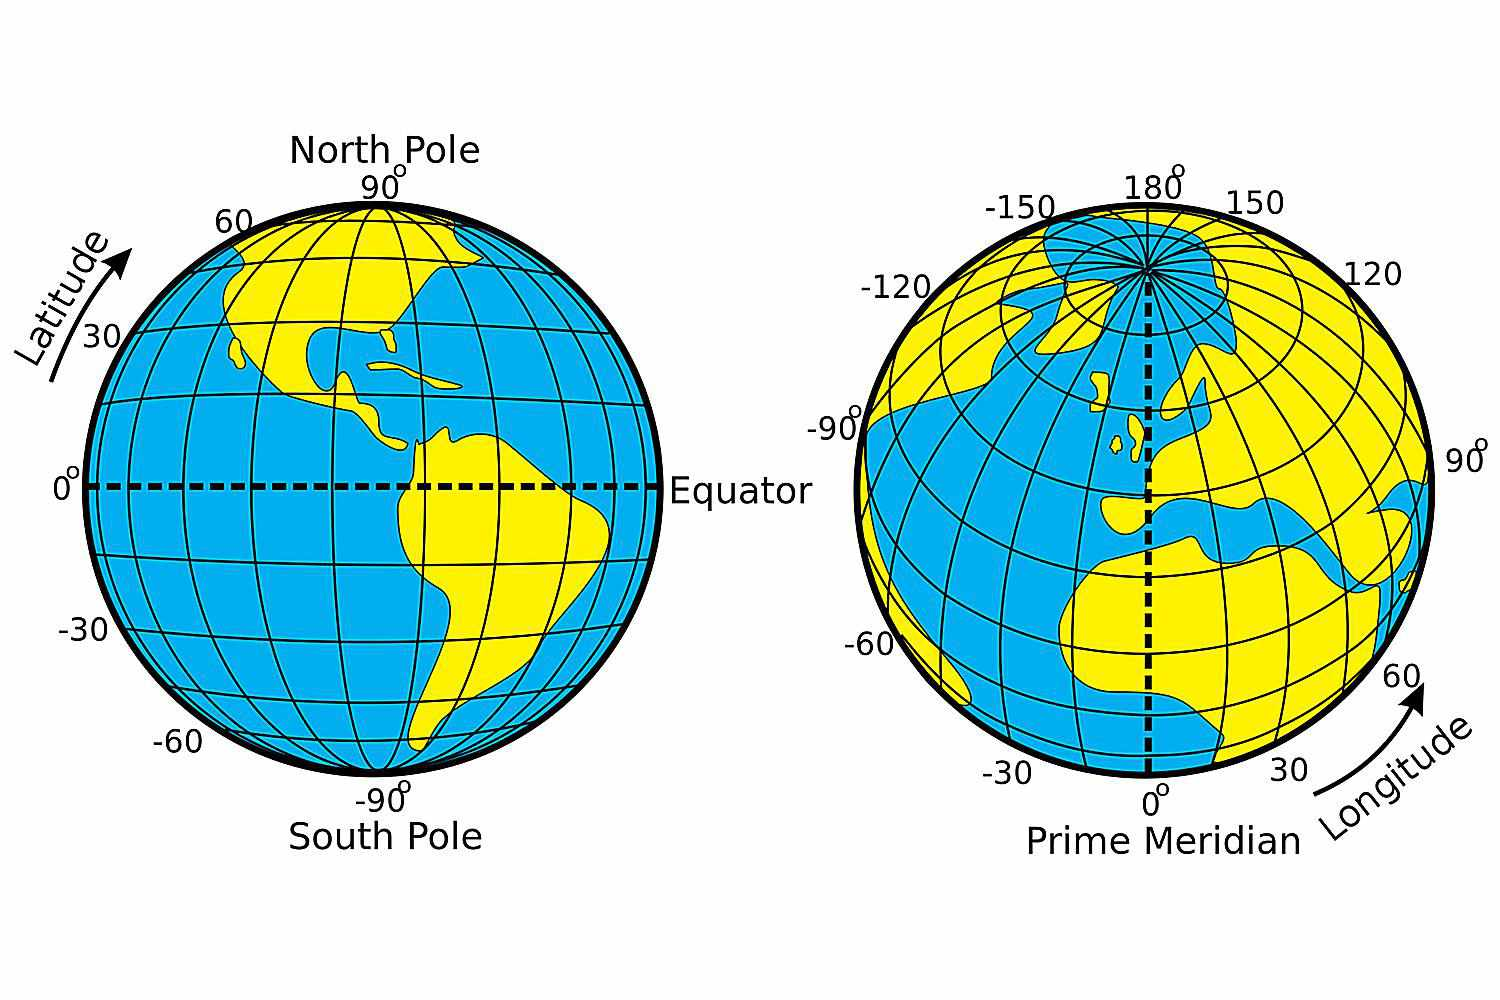
\includegraphics[width=0.5\textwidth]{C:/Users/Matteo/Shallow-Water-Equations/figs/lat-long-earth.jpg}
    \caption{Illustration of latitude and longitude on the planet earth.
    Illustration from~\cite{lat-long-earth}.}\label{fig:lat-long-earth}
\end{figure}
The spherical coordinates we use are ($r$, $\theta$, $\phi$), where $r$ is the radius from the center of the sphere, $\theta$ is the longitude, and $\phi$ is the latitude.
We also refer to $\theta$ as the elevation angle and $\phi$ as the azimuth angle, where $\phi$ goes from $-\frac{\pi}{2}$ at the south pole to $\frac{\pi}{2}$ at the north pole, calculated in radians.
The angle $\theta$ goes from $0$ at the priime meridian, increasing to the east, to $2\pi$ also calculated in radians.
In spherical coordinates any point on the surface of the sphere can be represented by the coordinates ($r$, $\theta$, $\phi$).
We consider a small domain of the sphere, as illustrated in \autoref{fig:sphere-small-domain}.
\begin{figure}[H]
    \centering
    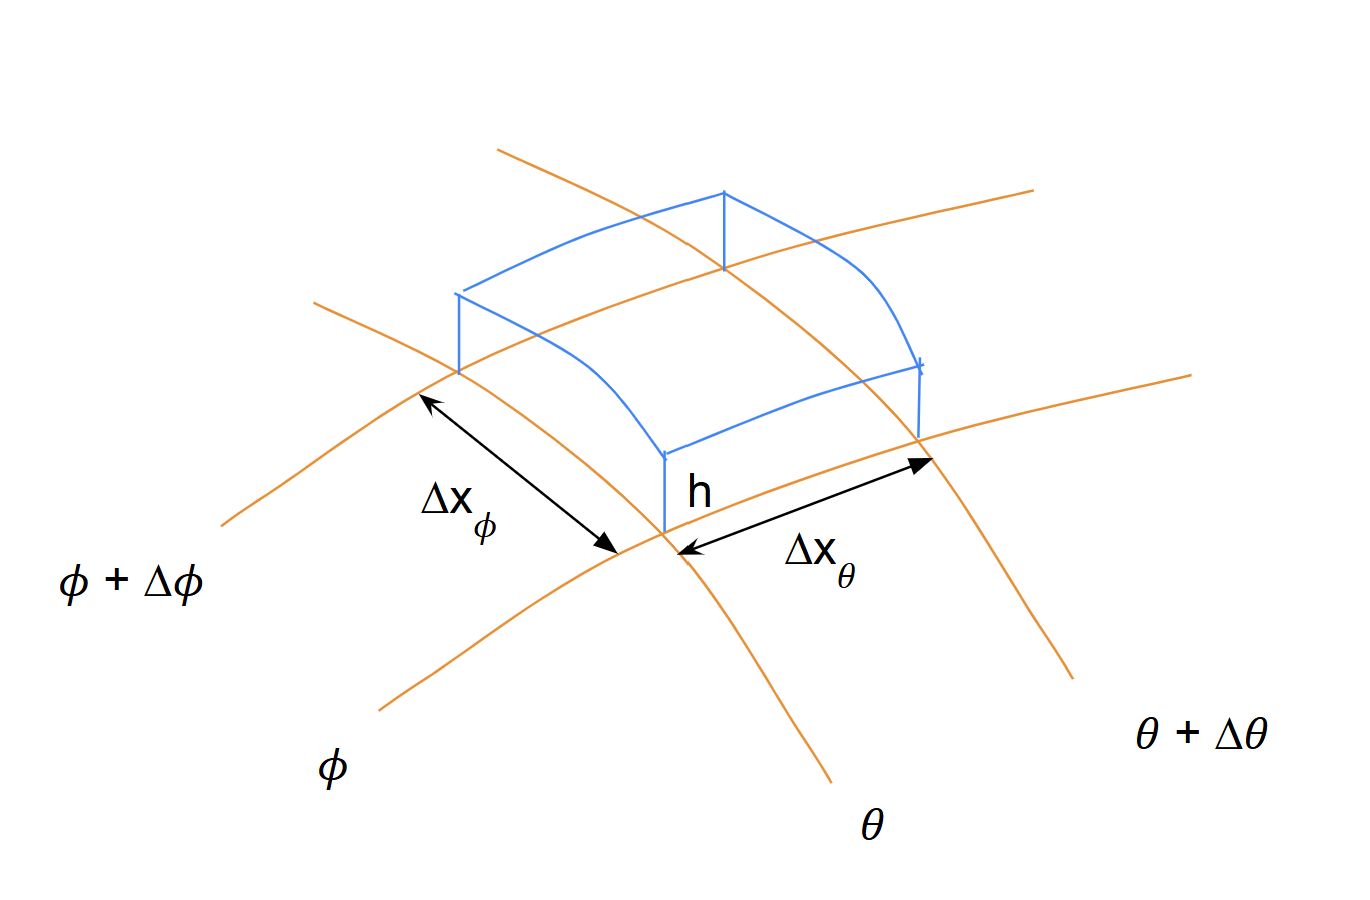
\includegraphics[width=0.5\textwidth]{C:/Users/Matteo/Shallow-Water-Equations/figs/Sphere-small-domain.png}
    \caption{Illustrations of a small domain of the surface of the sphere.}\label{fig:sphere-small-domain}
\end{figure}
We want to find expressions for $\Delta x_{\phi}$ and $\Delta x_{\theta}$, the distances in the $\phi$ and $\theta$ directions, respectively, as illustrated in \autoref{fig:sphere-small-domain}.
We can find these distances by using the arc length formula.
Recall that the circumreference of a full circle is $2\pi r$, where $r$ is the radius of the circle.
The arc length is a fraction of the full circumreference, and it is given by the formula $l = r v$, where $l$ is the arc length, $r$ is the radius, and $v$ is the angle in radians.
Assuming that the planet earth on the latitude side is a circle, we can find the distance $\Delta x_{\phi}$ by using the arc length formula, as:
\begin{align*}
    \Delta x_{\phi} = r \Delta \phi,
\end{align*}
where $\Delta \phi$ is the change in the latitude angle and $r$ is the radius of the sphere.
We assume that the planet earth is a perfect sphere, meaning that the radius is constant.
Considering the longitude dimension $\Delta x_{\theta}$, we need to make some adjustments, as we can see that the circumreference at equator is larger than at the poles.
Meaning that if we conisder the horizontal circle at some given latitude $\phi$, the radius of the circle is $r \cos(\phi)$ (why?).
Using that, together with the formula for the arc length, we can find the distance $\Delta x_{\theta}$ as:
\begin{align*}
    \Delta x_{\theta} = r \cos(\phi) \Delta \theta.
\end{align*}
The volume of a small domain of the sphere is given by 
\begin{align*}
    V &= \Delta x_{\phi} \Delta x_{\theta} h \\
    &= r^2 h \cos(\phi) \Delta \phi \Delta \theta,
\end{align*}
assuming that the height of the domain is $h$, and that the domain is rectangular.
This is a fair assumption for small values of $\Delta x_{\phi}$ and $\Delta x_{\theta}$.
We are interested in rate of change of the volume with respect to time, and we can find this by taking the time derivative of the volume.
That is, we consider the partial derivative with respect to time of the volume $V$:
\begin{align*}
    \frac{\partial V}{\partial t} &= r^2 \cos(\phi) \Delta \phi \Delta \theta \frac{\partial h}{\partial t},
\end{align*}
where we have utilized that $r$ is constant, and that $\cos(\phi), \Delta \phi$ and $\Delta \theta$ are independent of the time $t$.





The shallow water equations in spherical coordinates are given by:
\begin{equation}
    \left.
    \begin{aligned}
        h_t + \frac{1}{r \cos (\phi)} \left( {(h u_\theta)}_{\theta} {(h u_{\phi} \cos(\phi))}_{\phi}  \right) &= 0, \\
        {(u_{\theta})}_t  + \frac{u_\theta}{r \cos (\phi)} {(u_\theta)}_\theta + \frac{u_\phi}{r} {(u_\theta)}_{phi}
        - \frac{u_\theta u_\phi }{r} \tan(\phi) + \frac{g}{r \cos (\phi)} h_\theta &= \frac{g}{r \cos(\phi)} b_\theta, \\
        {(u_{\phi})}_t  + \frac{u_\theta}{r \cos (\phi)} {(u_\phi)}_\theta + \frac{u_\phi}{r} {(u_\phi)}_{\phi}
        + \frac{u_\theta^2}{r} \tan(\phi) + \frac{g}{r} h_\phi &= \frac{g}{r} b_\phi,
    \end{aligned}
    \right\}
\end{equation}
where $r$ is the radius, $(\theta, \phi)$ are the longitude and latitude, $h$ is the height of the water, $u_\theta$ and $u_\phi$ are the velocities in the $\theta$ and $\phi$ directions, $g$ is the gravitational constant, and $b$ is the bottom depth.






